\chapter{Cómputo bayesiano} \label{chap:Cap_MCMC}

De acuerdo con \textcite{Ross10}, los resultados más importantes y más conocidos de la teoría de probabilidad son los llamados teoremas límite, en particular aquellos conocidos como \textit{leyes de los grandes números}. La idea general podemos tomarla de Jakob Bernoulli, el primero en presentar un teorema de este tipo, y estriba en que todos los hombres saben ``por algún instinto de la naturaleza \textit{per se} y sin ninguna instrucción previa, que entre más observaciones hay, menor es el peligro de alejarse del blanco" \parencite{Pulskamp09}. Es decir, si tenemos suficientes realizaciones de un experimento, podemos estimar con mucha precisión aquello que buscamos.\\

Después de varios avances históricos que pueden consultarse en \textcite{Seneta13}, hoy contamos con las leyes débil y fuerte de los grandes números \parencite{Ross10}. Ambas nos dicen que, conforme el tamaño de una muestra aleatoria aumenta, los promedios empíricos convergen a los promedios teóricos. Una manera común de ejemplificar este fenómeno es mediante el lanzamiento sucesivo de monedas. En este caso los volados \textit{simulan} observaciones de una variable aleatoria de ensayos Bernoulli y, al tener una muestra suficientemente grande, se comienza a apreciar la convergencia hacia la probabilidad de éxito.\\ 

Gracias al avance tecnológico, hoy ya no tenemos necesariamente que lanzar volados físicamente sino que los simulamos desde una computadora, a partir de la generación de números pseudoaleatorios, diseñados de manera tal que satisfagan todas las propiedades básicas de números auténticamente aleatorios \parencite{Ross13}. Podemos pedirle a la computadora que simule una gran cantidad de volados \textit{justos} y registre la proporción empírica acumulada de los que cayeron águila. Conforme más aumenta el número de volados, más nos acercamos a 0.5, la proporción teórica. Esto se puede repetir para otras series de volados y el comportamiento es el mismo, como puede apreciarse en la \textbf{Figura \ref{fig:LGN}}. \\

\begin{figure}[h]
	\centering
	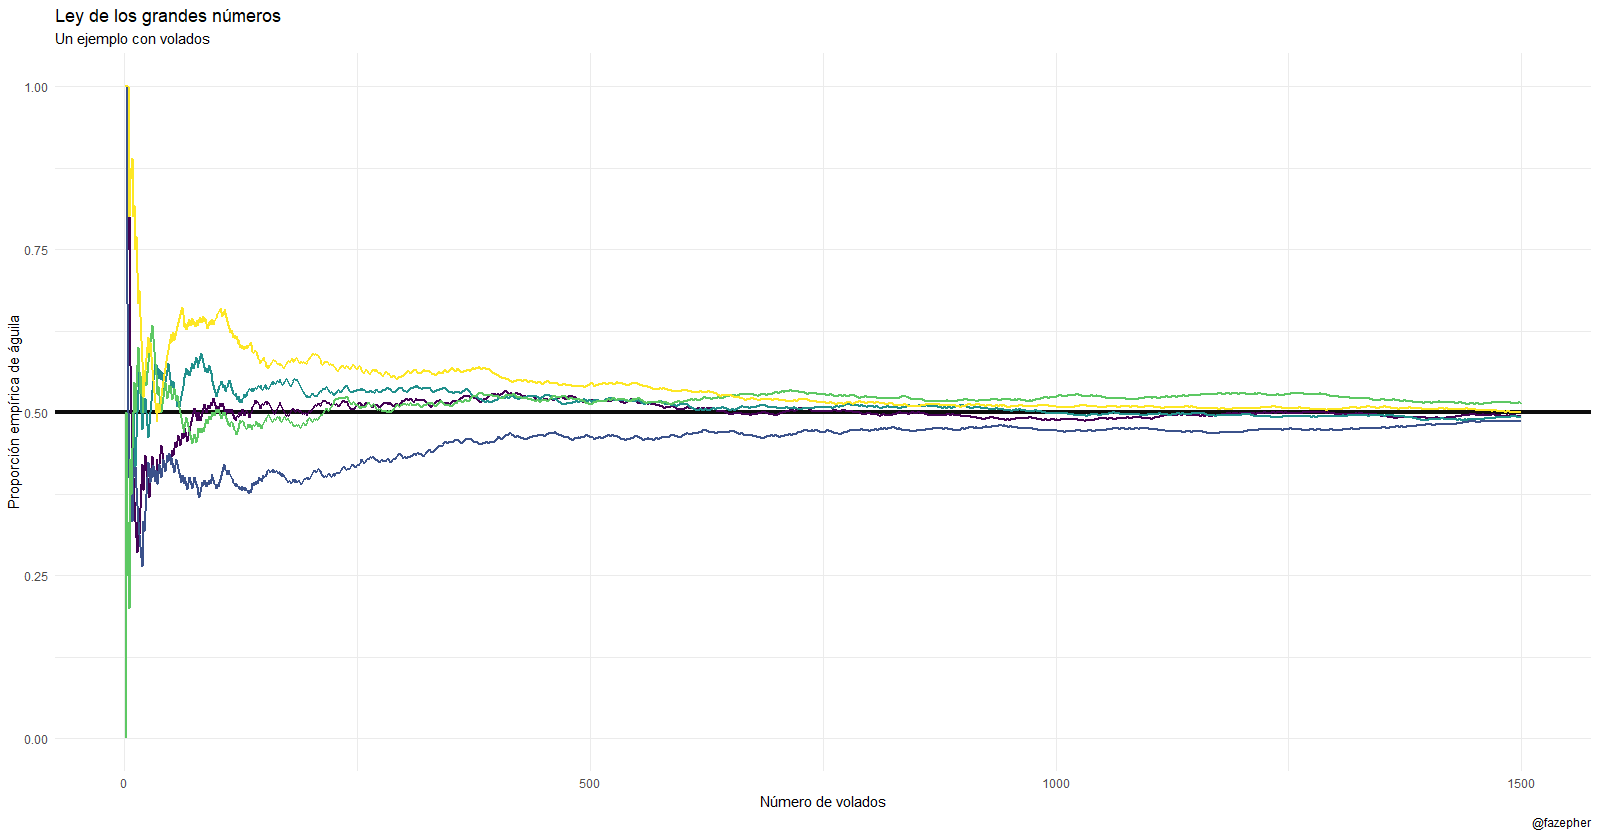
\includegraphics[scale=0.2]{Figs/LGN}
	\caption{Ilustración de las leyes de los grandes números mediante volados simulados por computadora. Conforme el número de volados aumenta, la proporción empírica converge a la proporción teórica. Esto pasa para cada serie de volados. Fuente: elaboración propia.}
	\label{fig:LGN}	
\end{figure}

Es cierto que esta práctica de aprender de un sistema, simulando con muestreo aleatorio no surge con las computadoras \parencite{Owen13}. Ya desde 1812 Laplace había sugerido la posibilidad de estimar empíricamente el valor de $\pi$ mediante el llamado problema de la aguja de Buffon \parencite{Ragheb13}. Sin embargo, como el ejemplo de los volados muestra, sí han sido las computadoras las que han potenciado la utilidad de los métodos de simulación. ¿Cuánto hubiéramos tardado en lanzar los 7,500 volados que la computadora simuló al instante? Más aún, esta capacidad computacional consolidó la utilidad de la estadística bayesiana. ¡Y pensar que todo empezó con una guerra y un juego de solitario!, como explico a continuación.

\section{Monte Carlo} 

La simulación por computadora ha permitido el desarrollo de la estadística bayesiana, particularmente desde la década de los 90 del siglo pasado \parencite{RobertCasella11}. Sin embargo, la semilla de este desarrollo ya había sido plantada medio siglo antes desde el terreno de la física, desafortunadamente a causa de la Segunda Guerra Mundial, por los científicos del laboratorio de Los Alamos, encargados del proyecto Manhattan y el desarrollo de más armas de fisión nuclear.\\

Uno de esos científicos fue un matemático polaco-estadounidense llamado Stanislaw Ulam. En 1946, aburrido convaleciendo por una enfermedad, comenzó a preguntarse sobre la probabilidad de ganar en un juego de solitario. Después de mucho batallar con los cálculos de combinatoria se planteó si no sería más práctico estimarla simulando muchas partidas en una de las primeras computadoras electrónicas. Y ahí surgió el eureka: ¿por qué no hacer lo mismo para los problemas de física nuclear en los que estaban trabajando en Los Alamos? \parencite{Eckhardt87}. Al igual que las partidas de solitario, podrían simular muchas realizaciones de los procesos físicos bajo estudio y estimar los resultados más probables.\\ 

Stan compartió su idea con John von Neumann quien, sorprendido y emocionado con la idea, le envió una carta a Richard Richtmayer--- el líder del equipo en Los Alamos--- con todos los cálculos necesarios para llevar a cabo el proyecto \parencite{vonNeumann47}. El método fue rápidamente adoptado por todos en Los Alamos, tanto que otro físico, Nicholas Metropolis, sugirió llamarlo \textit{Monte Carlo}, bromeando sobre un tío apostador de Stan, que vivía pidiendo prestado dinero porque ``simplemente tenía que ir a Monte Carlo" \parencite{Metropolis87}. Después de un arduo trabajo, el método pareció funcionar--- gracias en buena medida al trabajo de programación de Klara von Neumann \parencite{Haigh14}--- y el propio Metropolis publicó, junto con Stan, un primer paper presentándolo a grandes rasgos \parencite{MetropolisUlam49}.\\

De manera concreta, el método es la conjunción de la simulación con la ley de los grandes números. Las cantidades que requerían calcular eran valores esperados de la siguiente forma: 
\begin{equation}
\label{eq:IntegralMC}
h^\star = \mathbb{E}[h(Z)]=\int\limits_\mathcal{Z} h(z)f(z)dz ,
\end{equation} 
donde $h$ es una función de interés y $f(z)$ es la distribución de probabilidad sobre las \textit{configuraciones} $z$ en las que podía encontrarse el sistema físico. El gran problema era--- y sigue siendo--- que estas integrales típicamente no pueden calcularse ni analíticamente ni por métodos numéricos tradicionales. Sin embargo, si se tiene una muestra aleatoria de valores de $Z$ provenientes de su distribución $f$, se puede aproximar $h^\star$ con el promedio empírico, que en este contexto se conoce como \textit{estimador de Monte Carlo}: 
\begin{equation*}
h^\star \approx \hat{h} = \sum\limits_{i=1}^N \dfrac{h(z_i)}{N}
\end{equation*}

Entonces, los científicos en Los Alamos se dedicaron a encontrar algoritmos eficientes para obtener una muestra aleatoria de variables provenientes de diferentes distribuciones $f$.\\ 

Lo importante para este trabajo es que este es exactamente el mismo probelma que se tiene en la aplicación de la estadística bayesiana y que hizo que por décadas--- por no decir siglos--- fuera poco menos que imposible llevar a cabo análisis bayesianos no triviales, como ya anticipa en \ref{sec:Prob_Analitico}. En efecto, las integrales que surgen en la estadística bayesiana no pueden ser calculadas de manera analítica. El ejemplo más frecuente es la constante normalizadora del teorema de Bayes. ¿Cómo aplicar el teorema si el denominador no puede ser calculado?\\ 

No obstante, la forma de \eqref{eq:IntegralMC} permite llevar a cabo una gran variedad de \textit{resúmenes inferenciales} \parencite{GP97}. La posibilidad de realizar la correspondiente \textit{integración por Monte Carlo} hace que, en la práctica, exista una dualidad entre una distribución o densidad y una muestra proveniente de ella \parencite{SmithGelfand92}. La única receta de la inferencia bayesiana--- ver la página \pageref{receta_bayesiana}---, en la práctica se convierte en obtener una muestra aleatoria de la distribución posterior lo suficientemente grande para, con ella, estimar por Monte Carlo los resúmenes inferenciales requeridos.\\

Hay varios métodos de simulación de variables aleatorias que permiten obtener muestras aleatorias independientes y calcular un estimador de Monte Carlo. Entre los más mencionados podemos encontrar el método de inversión, el de aceptación y rechazo o el muestreo por importancia \parencites{Ross13,RobertCasella10}. Sin embargo, los físicos de Los Alamos pronto se dieron cuenta que, en lugar de buscar realizar directamente simulaciones independientes, podrían hacer simulaciones secuenciales que dependieran entre sí. 

\section{MCMC}

La forma de realizar simulaciones correlacionadas que logren simular de manera más eficiente que los métodos directos tradicionales de aceptación y rechazo o muestreo por importancia es utilizar \textit{cadenas de Markov}.

\dfn{\textbf{Cadena de Markov}\\
\label{def:Cadena_Markov}
Una \textit{cadena de Markov} $\left\lbrace Z_{(n)}, \, n = 0, 1, 2,\dots \right\rbrace$ es una secuencia de variables aleatorias tales que satisfacen la siguiente \textit{propiedad de Markov} para toda $n$
\begin{equation*}
Z_{(n+1)}| Z_{(n)}, \dots, Z_{(0)} \sim Z_{(n+1)}| Z_{(n)} \sim p(z_{(n+1)}|z_{(n)})
\end{equation*}
}
Si llamamos \textit{estados} a los eventos que suceden en la cadena en cada punto en el tiempo, podemos decir que la distribución condicional del estado futuro de una cadena de Markov dada toda su historia depende exclusivamente del estado presente y no de los estados anteriores. Dicho de otra forma, \textit{el futuro es independiente del pasado, dado el presente}. La distribución condicional se llama \textit{kernel de transición}, mismo que normalmente es también independiente del índice $n$ y depende exclusivamente del estado actual y el estado futuro. Esta propiedad se llama \textit{homogeneidad} en el tiempo y permite simplificar la notación a $p(\tilde{z}|z)$.\\ 

La teoría de cadenas de Markov determina las condiciones bajo las cuales existen teoremas límites al estilo de las leyes de los grandes números y que en este contexto se conocen como \textit{ergódicos}. Esta teoría escapa los objetivos particulares de la tesis pero, si es de interés para el lector, algunas referencias útiles son \textcites{Rincon12,Neal93,Ross96,TaylorKarlin84}. Baste decir por ahora que, bajo ciertas condiciones, sabemos que la distribución de $Z_{(n)}$ converge a una distribución límite conforme $n$ tiende a infinito. Más aún, los \textit{promedios ergódicos}--- es decir los promedios acumulados de la cadena--- también convergen al valor esperado de la distribución límite. Esto se puede expresar matemáticamente como sigue:
\begin{subequations}\label{eq:Teo_Erg}
\begin{align}
Z_{(N)} &\xrightarrow[N\rightarrow\infty]{\mathcal{D}} Z, \quad Z \sim f(z) \label{eq:Teo_Erg_Conv_D} \\
\dfrac{1}{N}\sum\limits_{n=1}^N h(z_{(n)}) &\xrightarrow[N\rightarrow\infty]{} E_{f}[h(z)]
\label{eq:Teo_Erg_Conv_Prom}
\end{align}
\end{subequations}

Esto da lugar a los métodos de \textit{Markov Chain Monte Carlo} o MCMC en los que el objetivo es construir una cadena de Markov que satisfaga las condiciones necesarias y cuya distribución límite sea la distribución de la cual se quiere simular. Así, después de $N$ transiciones de la cadena, la cadena de valores simulados convergería a la distribución objetivo y se podría estimar la cantidad de interés $h^\star$ mediante el estimador de MCMC: 

\begin{equation*}
h^\star \approx \hat{h} = \sum\limits_{n=1}^N \dfrac{h(z_{(n)})}{N}
\end{equation*}

\subsection{Metropolis Hastings}

 El primero de estos métodos MCMC fue propuesto por las parejas de esposos Arianna y Marshall Rosenbluth y Augusta y Edward Teller junto con el propio Nicholas Metropolis en el \textit{Journal of Chemical Physics} \parencite{Metropolis53}. Se conoce como el algoritmo de Metropolis, aunque hay quienes creen que en realidad el trabajo más fuerte lo hicieron el resto de los autores por lo que debería llamarse el algoritmo de Rosenbluth-Teller \parencite{Gubernatis05}. Casi 20 años después, el estadístico canadiense Wilfred Keith Hastings lo generalizó \parencite{Hastings70}, por lo que podemos hablar de algoritmos de Metropolis Hastings o MH.

\subsubsection*{Balance detallado, la clave de MH}
 
Las cadenas de Markov para MH requieren ser homogéneas en el tiempo y que sea posible llegar a cualquier estado en un número finito de transiciones, algo que se conoce como \textit{irreducibilidad}. Si además el kernel de transición satisface la siguiente \textit{ecuación de balance detallado} para alguna distribución $f$, se dice que es \textit{reversible} y podemos aplicar el teorema ergódico.
\begin{equation}
\label{eq:Balance_Detallado}
f(z)p(\tilde{z}|z)=f(\tilde{z})p(z|\tilde{z})
\end{equation}

El algoritmo de Metropolis Hastings busca construir cadenas de Markov homogéneas, irreducibles y reversibles que tengan como distribución límite a la distribución objetivo. ¿Cómo hacerlo? Para ello analicemos lo que la reversibilidad implica de manera intuitiva.\\

Siguiendo la argumentación de \textcite{ChibGreenberg95}, \eqref{eq:Balance_Detallado} refleja que hay un balance entre las probabilidades de la cadena de estar en diferentes estados, de ahí el nombre. Supongamos que no se cumpliera la reversibilidad para algún kernel $q(\tilde{z}|z)$. Entonces, sin pérdida de generalidad, para algunos estados pasaría que:
\begin{equation}
\label{eq:Inbalance_Detallado}
\dfrac{f(z)}{f(\tilde{z})}>\dfrac{q(z|\tilde{z})}{q(\tilde{z}|z)}
\end{equation}

De manera un poco informal, tenemos que el miembro izquierdo de la desigualdad refleja las probabilidades relativas ``necesarias'' entre estar en el estado $z$ y el estado $\tilde{z}$. El miembro derecho, por su parte, indica las probabilidades relativas de transitar a dichos estados bajo el kernel de transición de la cadena. La desigualdad indica que la cadena estaría transitando a $\tilde{z}$ más de lo necesario y, equivalentemente, transitaría a $z$ menos de lo necesario.\\ 

Para conseguir el balance requerido para aplicar el teorema ergódico, necesitamos hacer una \textit{corrección de Metropolis} al kernel de transición, reduciendo el número relativo de veces que la cadena transite de $z$ a $\tilde{z}$ y aumentando el número relativo de transiciones de $\tilde{z}$ a $z$. La forma de hacer la corrección es comenzar con un kernel, $q(\tilde{z}|z)$, que \textit{proponga} un estado y agregar una \textit{probabilidad de aceptación} de la propuesta, $\alpha(\tilde{z};z)$. Si es rechazada, la cadena permanece en el mismo estado, reduciendo a la vez el número de transiciones hacia estados sobremuestreados y aumentando el número relativo de veces que estamos en el estado originalmente submuestreado. Estos dos pasos constituyen un kernel de transición de Metropolis Hastings de la siguiente forma: 
\begin{align*}
p_{MH}(\tilde{z}|z) &= q(\tilde{z}|z)\alpha(\tilde{z};z) \quad z \neq \tilde{z} \\
p_{MH}(z|z) &= 1 - \int\limits_{\tilde{\mathcal{Z}}} p_{MH}(\tilde{z}|z)d\tilde{z}
\end{align*}

Queremos que el kernel $p_{MH}$ satisfaga \eqref{eq:Balance_Detallado}, entonces:
\begin{equation*}
f(z)p_{MH}(\tilde{z}|z)=f(\tilde{z})p_{MH}(z|\tilde{z}) \quad \Leftrightarrow \quad f(z)q(\tilde{z}|z)\alpha(\tilde{z};z)=f(\tilde{z})q(z|\tilde{z})\alpha(z;\tilde{z}) 
\end{equation*}

De acuerdo a nuestra desigualdad supuesta en \eqref{eq:Inbalance_Detallado}, las transiciones de $\tilde{z}$ a $z$ se dan demasiado poco, por lo que deberíamos siempre aceptar este tipo de transiciones a fin de corregir el submuestreo. Tomemos entonces $\alpha(z;\tilde{z}) = 1$ y observemos que $\alpha(\tilde{z};z)$ queda determinada de tal forma que logremos el balance necesario: 
\begin{equation*}
\alpha(\tilde{z};z)=\dfrac{f(\tilde{z})q(z|\tilde{z})}{f(z)q(\tilde{z}|z)}
\end{equation*}

Si la desigualdad \eqref{eq:Inbalance_Detallado} fuera en el sentido contrario, i.e. $f(\tilde{z})q(z|\tilde{z})>f(z)q(\tilde{z}|z)$, los roles de las probabilidades de aceptación se invertirían, por lo que de manera general tenemos que 
\begin{equation}
\label{eq:Proba_Aceptar_MH}
\alpha(\tilde{z};z)=min\left\lbrace\dfrac{f(\tilde{z})q(z|\tilde{z})}{f(z)q(\tilde{z}|z)},1\right\rbrace
\end{equation}

La utilidad de MH para la estadística bayesiana está en la forma \eqref{eq:Proba_Aceptar_MH} de la probabilidad de aceptación. Como la distribución objetivo se encuentra tanto en el denominador como en el numerador, no se requiere completa sino basta con conocerla salvo por una constante de proporcionalidad que desaparezca al realizar el cociente. Esta situación es exactamente la que impera en la aplicación de la estadística bayesiana. Recordemos el resumen del aprendizaje bayesiano en \eqref{eq:Bayes_Prop}, \textit{la posterior es proporcional a la inicial por la verosimilitud}: 
\begin{equation*}
f(\theta|y) \propto L(\theta)f(\theta).
\end{equation*}

Por esto, para simular valores de una distribución posterior $f(\theta|y)$ mediante MH solo necesitamos la distribución inicial $f(\theta)$, la verosimilitud $L(\theta)=f(y|\theta)$ y un kernel de propuestas $q(\tilde{\theta}|\theta)$, siguiendo el \textbf{Algoritmo \ref{alg:MH}}. Hay una última consideración que debe tenerse en cuenta y es que la posterior sea propia; si se inició con una inicial impropia es posible que la posterior no pueda integrar a 1, lo que haría que el algoritmo fallara \parencite{RobertCasella10}.\\

\begin{algorithm}
\DontPrintSemicolon
Valor inicial arbitrario o simulado $\theta_{(0)}$\;
\For{$n \leftarrow 1$ \KwTo $N$}{
$\theta \leftarrow \theta_{(n-1)}$\;
$\tilde{\theta} \sim q(\tilde{\theta}|\theta)$\;
$\alpha(\tilde{\theta};\theta) \leftarrow min\left\lbrace\dfrac{f(y|\tilde{\theta})f(\tilde{\theta})q(\theta|\tilde{\theta})}{f(y|\theta)f(\theta)q(\tilde{\theta}|\theta)},1\right\rbrace$\;
$u \sim U[0,1]$ \;
\eIf{$u \leq \alpha(\tilde{\theta};\theta)$}{
	$\theta_{(n)} \leftarrow \tilde{\theta}$\;
	}{
	$\theta_{(n)} \leftarrow \theta $\;
	}
}

\caption{Metropolis Hastings para el aprendizaje bayesiano \label{alg:MH}}
\end{algorithm}

\subsubsection*{\textit{Random Walk Metropolis}}

Si la posterior es propia, entonces el mayor problema, claro está, es el de encontrar un kernel de propuestas conveniente. Una alternativa son aquellos que exploran progresivamente el espacio de estados de manera local. Estos se conocen como \textit{Random Walk Metropolis} o RWM \parencite{RobertCasella10}. De hecho, el algoritmo inicial de \textcite{Metropolis53} era de este tipo, usando una distribución uniforme en una vecindad del estado actual; pero también se pueden usar otras distribuciones, como una normal o una $t$ de Student centrada en dicho estado. \textcite{Robert15} hace la analogía con alguien que para ver una pintura en un cuarto oscuro tiene que ir alumbrando el cuadro con una antorcha, iluminando secuencialmente diferentes segmentos del lienzo.\\

Estos kérneles de caminata aleatoria son \textit{simétricos}--- esto es,  $q(\tilde{\theta}|\theta) = q(\theta |\tilde{\theta})$--- lo que simplifica los cálculos de probabilidades de aceptación:
\begin{equation*}
\alpha_{RWM}(\tilde{\theta};\theta)=min\left\lbrace\dfrac{f(\tilde{\theta}|y)q(\theta|\tilde{\theta})}{f(\theta|y)q(\tilde{\theta}|\theta)},1\right\rbrace = min\left\lbrace\dfrac{f(\tilde{\theta}|y)}{f(\theta|y)},1\right\rbrace
\end{equation*}

Un ejemplo trivial puede ayudar a visualizar cómo funcionan. Supongamos que quisiéramos simular de una posterior que, en realidad, es una normal bivariada cuyas marginales son normales estándar. Un posible kernel de transición sería una distribución uniforme en un rectángulo de $3$ de lado centrado en el estado actual de la cadena, por lo que tendríamos un kernel simétrico y un algoritmo de \textit{Random Walk Metropolis}.\\ 

Podemos ver cómo se va explorando el espacio de estados en la \textbf{Figura \ref{fig:RWM}}. Cuando una de las propuestas es rechazada, esta se marca como una tache. Empezando en un punto alejado del origen, la cadena comienza a acercarse a la región de mayor densidad. En el fondo, encontrar esta \textit{región crítica} y explorarla--- obteniendo una muestra cada vez más fiel de la distribución--- es el objetivo de un algoritmo de integración por MCMC \parencites{Neal93,Betancourt17}. Con tan solo 2,500 iteraciones la cadena ya la recorrió y los valores que alejarían a la cadena de la misma son normalmente rechazados. Podemos ver también cómo los promedios ergódicos van acercándose a $0$ para ambas variables.\\

\begin{figure}[h]
    \centering
    \begin{subfigure}{0.3\textwidth}
        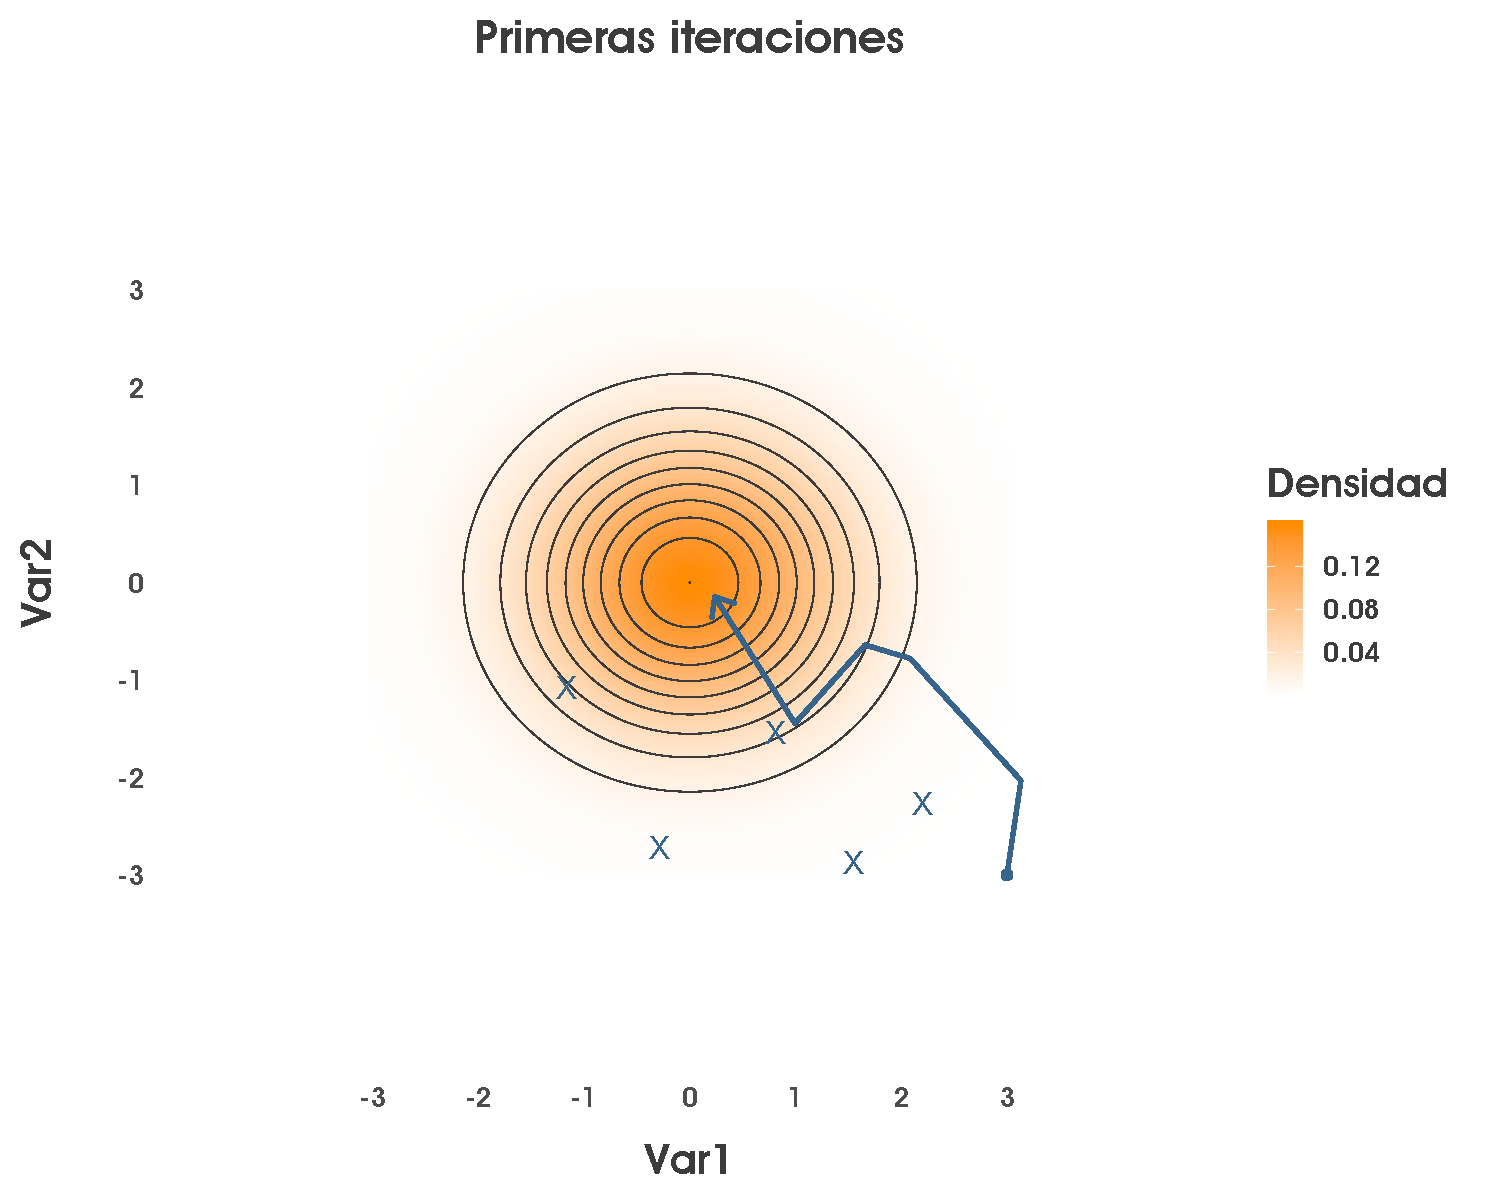
\includegraphics[width=\textwidth]{Figs/Bayes/Ejemplo_RWM_A}
        \caption{La cadena empieza lejos de las zonas de mayor densidad y se va acercando a ellas. Las taches representan propuestas rechazadas.}
    \end{subfigure}
    ~ 
    \begin{subfigure}{0.3\textwidth}
        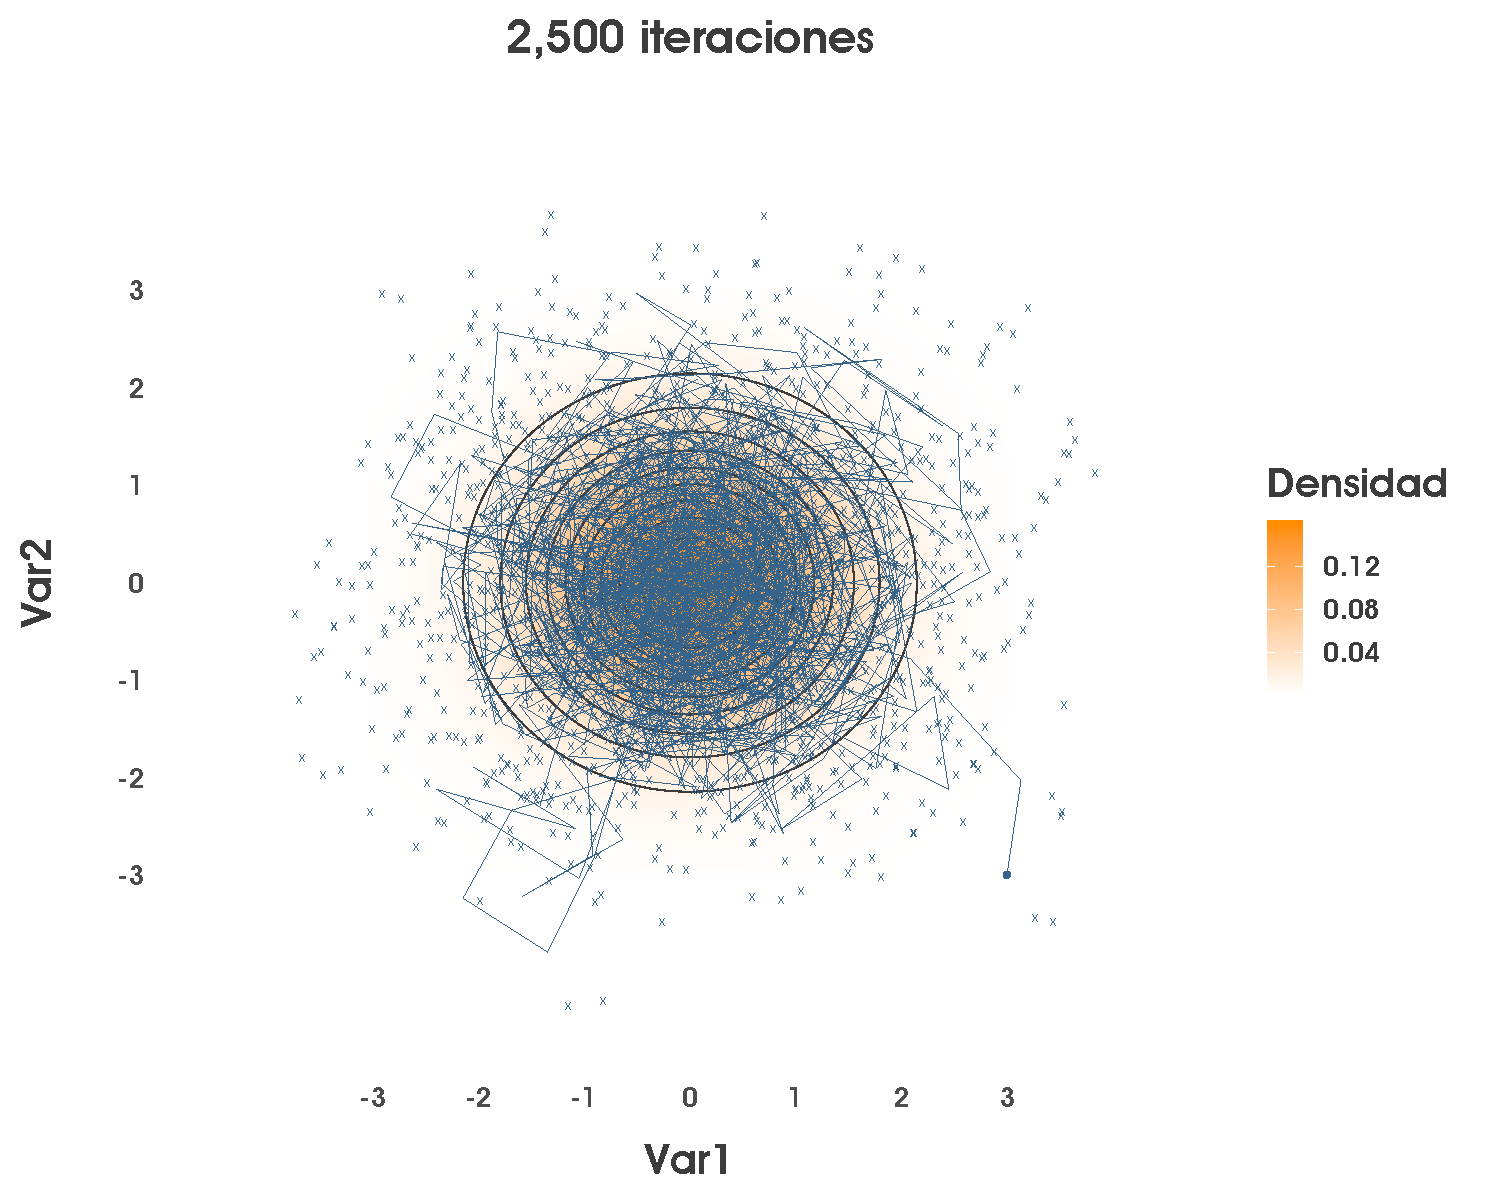
\includegraphics[width=\textwidth]{Figs/Bayes/Ejemplo_RWM_B}
        \caption{Después de 2,500 iteraciones, la cadena explora ya la región crítica. Los valores fuera de ella normalmente son rechazados.}
    \end{subfigure}
    ~
    \begin{subfigure}{0.3\textwidth}
        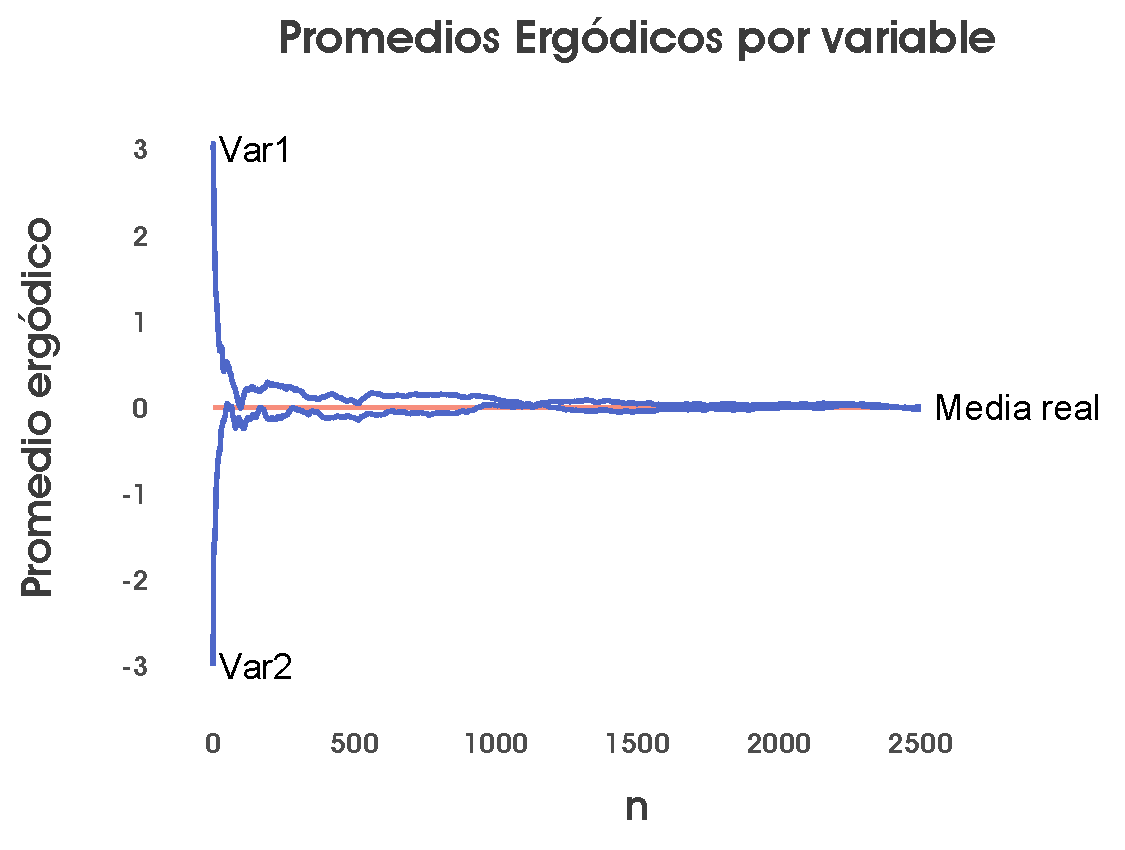
\includegraphics[width=\textwidth]{Figs/Bayes/Ejemplo_RWM_C}
        \caption{Los promedios ergódicos van convergiendo a las medias teóricas.}
    \end{subfigure}
    \caption{Ilustración de una cadena de Metropolis Hastings simulando de una normal bivariada sin correlación mediante una implementación de \textit{Random Walk Metropolis}. Fuente: elaboración propia.}\label{fig:RWM}
\end{figure}

La convergencia de los promedios ergódicos que implica \eqref{eq:Teo_Erg_Conv_Prom} es ciertamente importante. Sin embargo, en un análisis bayesiano la única receta indica tener una muestra aleatoria de la distribución posterior. Si observamos con cuidado \eqref{eq:Teo_Erg_Conv_D}, vemos que es la última simulación de la cadena la que podemos considerarla como proveniente de la distribución objetivo límite.\\

Pero la pregunta permanece, ¿cómo determinar el kernel de propuestas? ¿Por qué usar $3$ como lado y no $0.5$? ¿Qué hubiera pasado en ese caso? Podemos observarlo en la \textbf{Figura \ref{fig:RWM2}}. El rectángulo es más pequeño y eso tiene dos efectos: hay menos propuestas rechazadas pero la cadena avanza más lentamente. Vemos cómo aún después de las mismas 2,500 iteraciones la cadena no ha explorado por completo el área de mayor densidad y los promedios ergódicos apenas comienzan a converger.\\ 

\begin{figure}[h]
    \centering
    \begin{subfigure}{0.3\textwidth}
        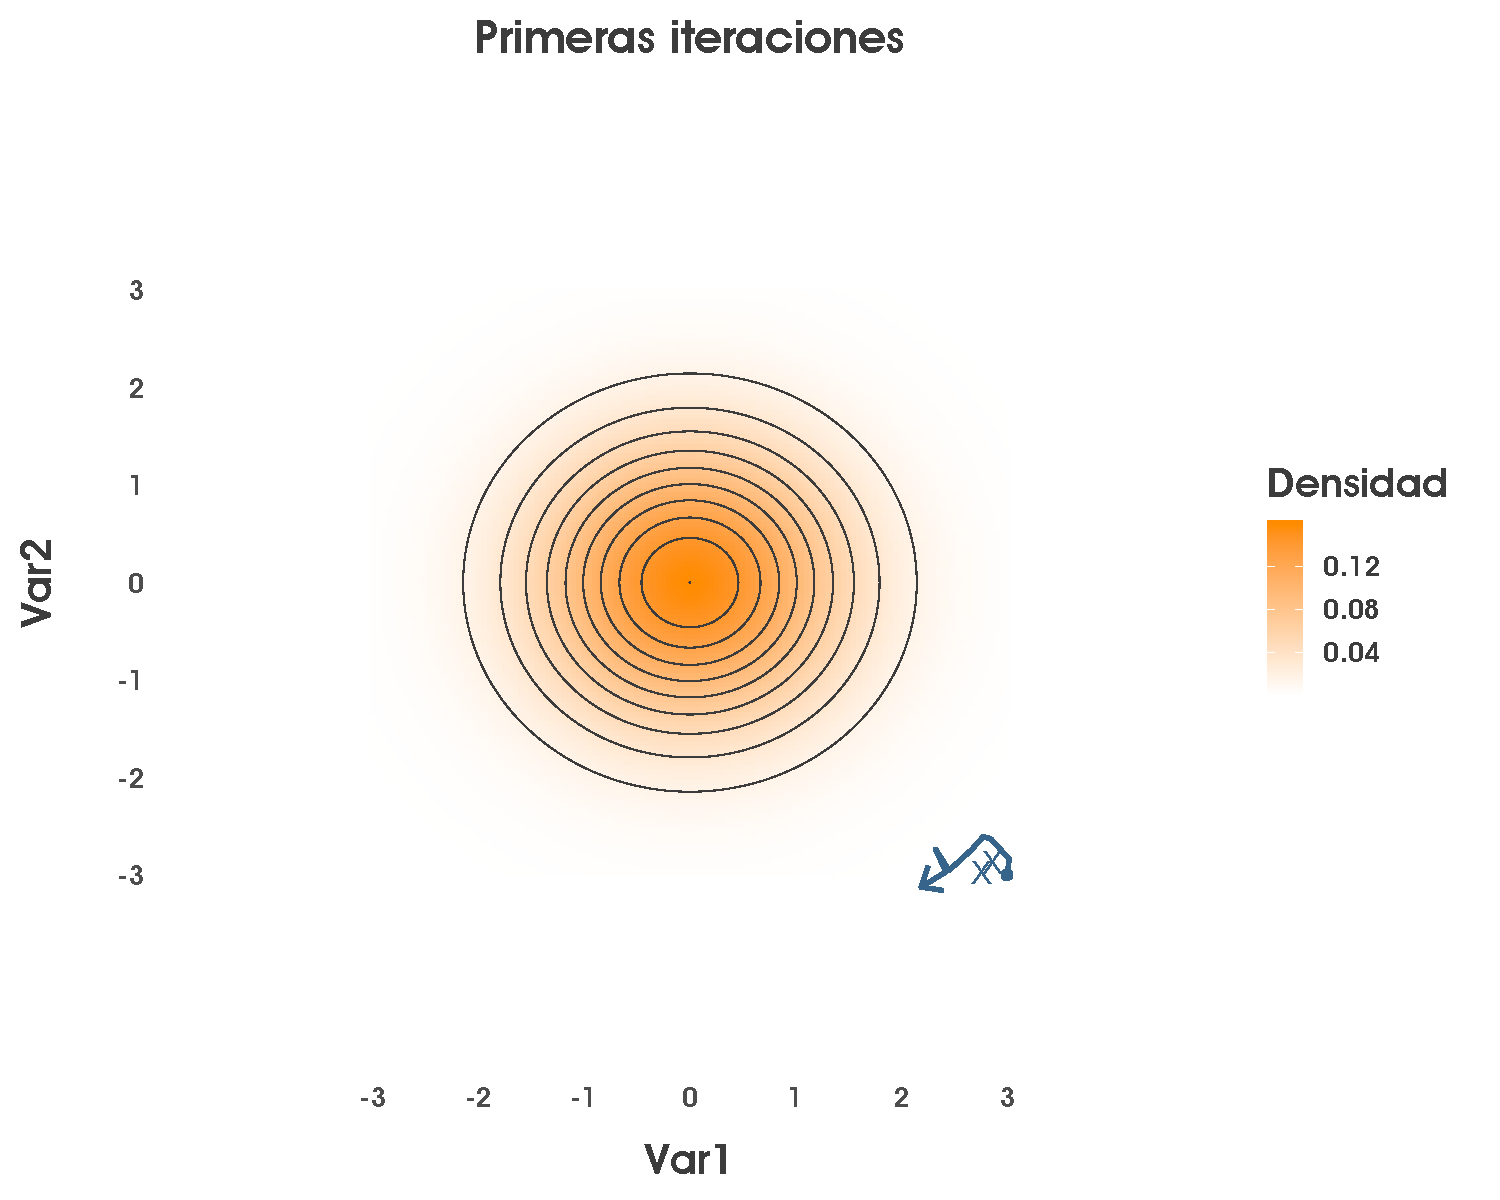
\includegraphics[width=\textwidth]{Figs/Bayes/Ejemplo2_RWM_A}
        \caption{La cadena empieza lejos de las zonas de mayor densidad y avanza lentamente. Las taches representan propuestas rechazadas.}
    \end{subfigure}
    ~ 
    \begin{subfigure}{0.3\textwidth}
        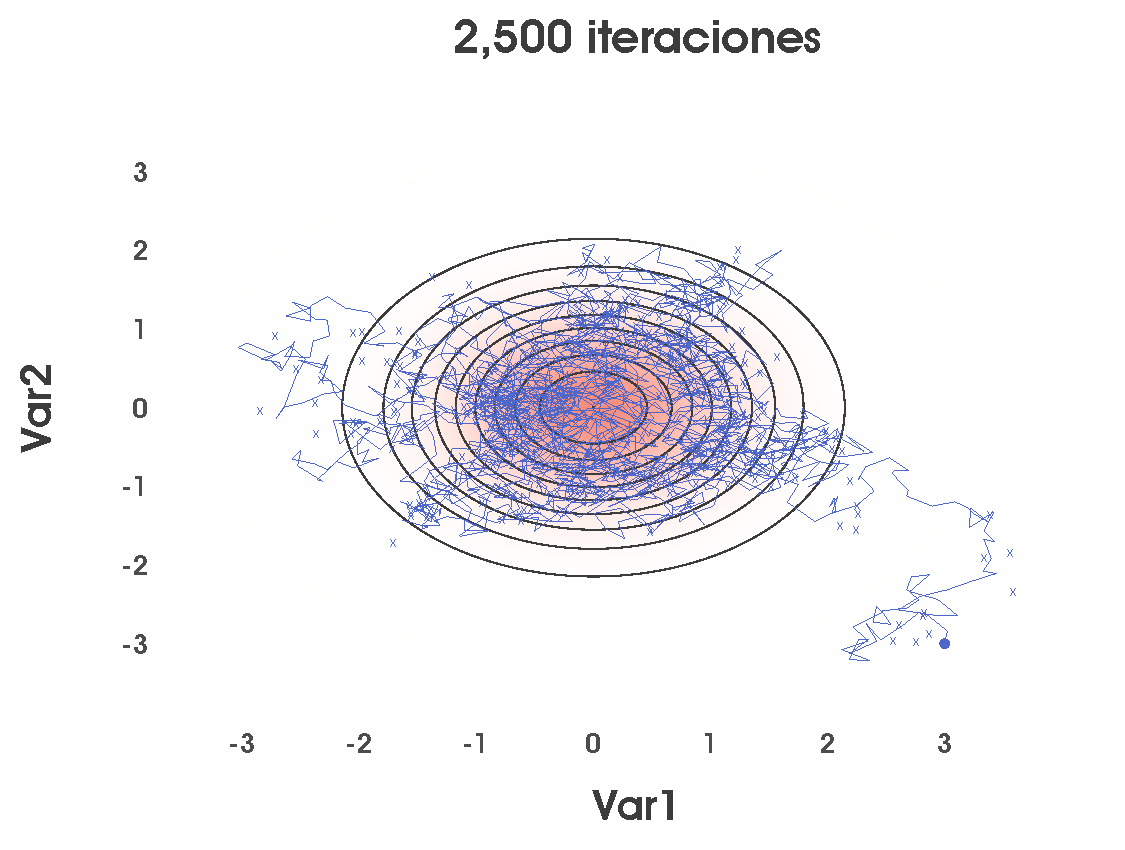
\includegraphics[width=\textwidth]{Figs/Bayes/Ejemplo2_RWM_B}
        \caption{Después de 2,500 iteraciones, la cadena no ha explorado la región crítica, aunque hay menos propuestas rechazadas.}
    \end{subfigure}
    ~
    \begin{subfigure}{0.3\textwidth}
        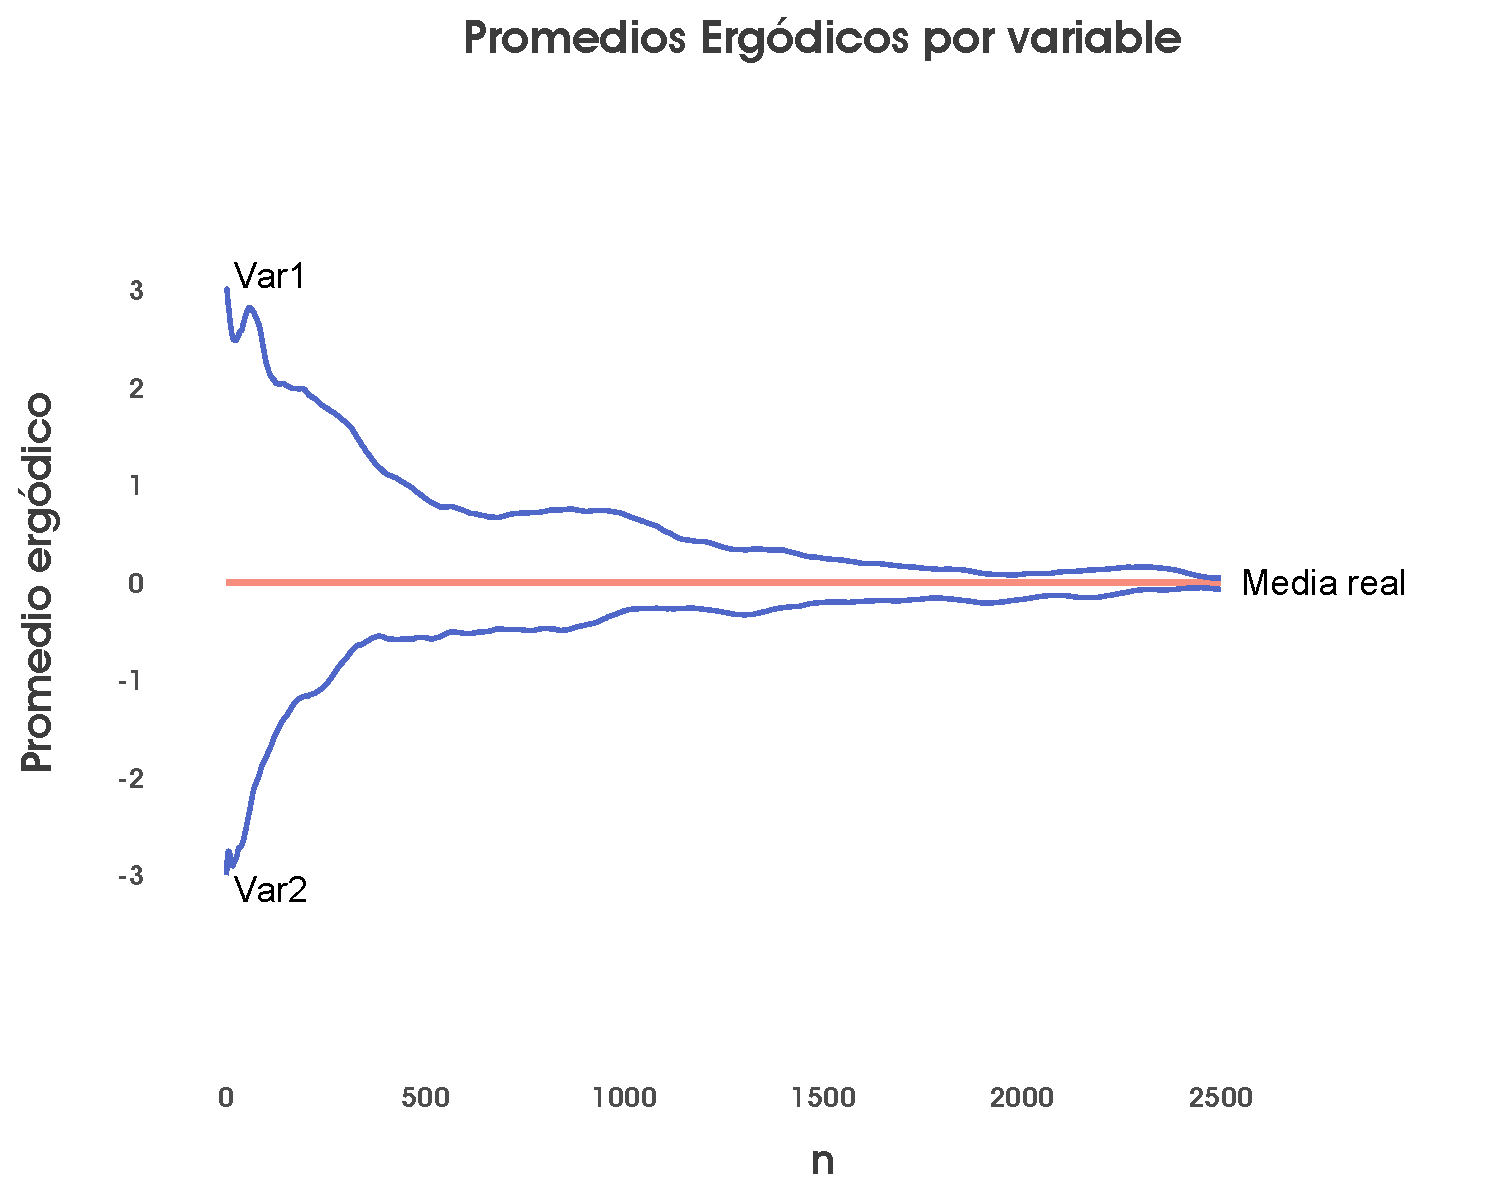
\includegraphics[width=\textwidth]{Figs/Bayes/Ejemplo2_RWM_C}
        \caption{Los promedios ergódicos tardan en converger.}
    \end{subfigure}
    \caption{Ilustración de una cadena de Metropolis Hastings simulando de una normal bivariada sin correlación mediante una implementación de \textit{Random Walk Metropolis} con un kernel de propuestas estrecho. Fuente: elaboración propia.}\label{fig:RWM2}
\end{figure}

Este comportamiento puede no ser el deseado en el ejemplo, pero es importante tenerlo en cuenta. El rectángulo más amplio permite proponer valores más distantes del punto actual, lo que en este caso hace que la cadena avance rápidamente. Sin embargo, también propone valores que se alejan de la región crítica, mismos que tienden a ser rechazados. El rectángulo más pequeño avanza más bien ``lento pero seguro''. Esto podemos verlo comparando el comportamiento de ambos kérneles cuando intentan simular normales ahora altamente correlacionadas, en la \textbf{Figura \ref{fig:RWM_Corr}}.\\

\begin{figure}[h]
    \centering
    \begin{subfigure}{0.3\textwidth}
        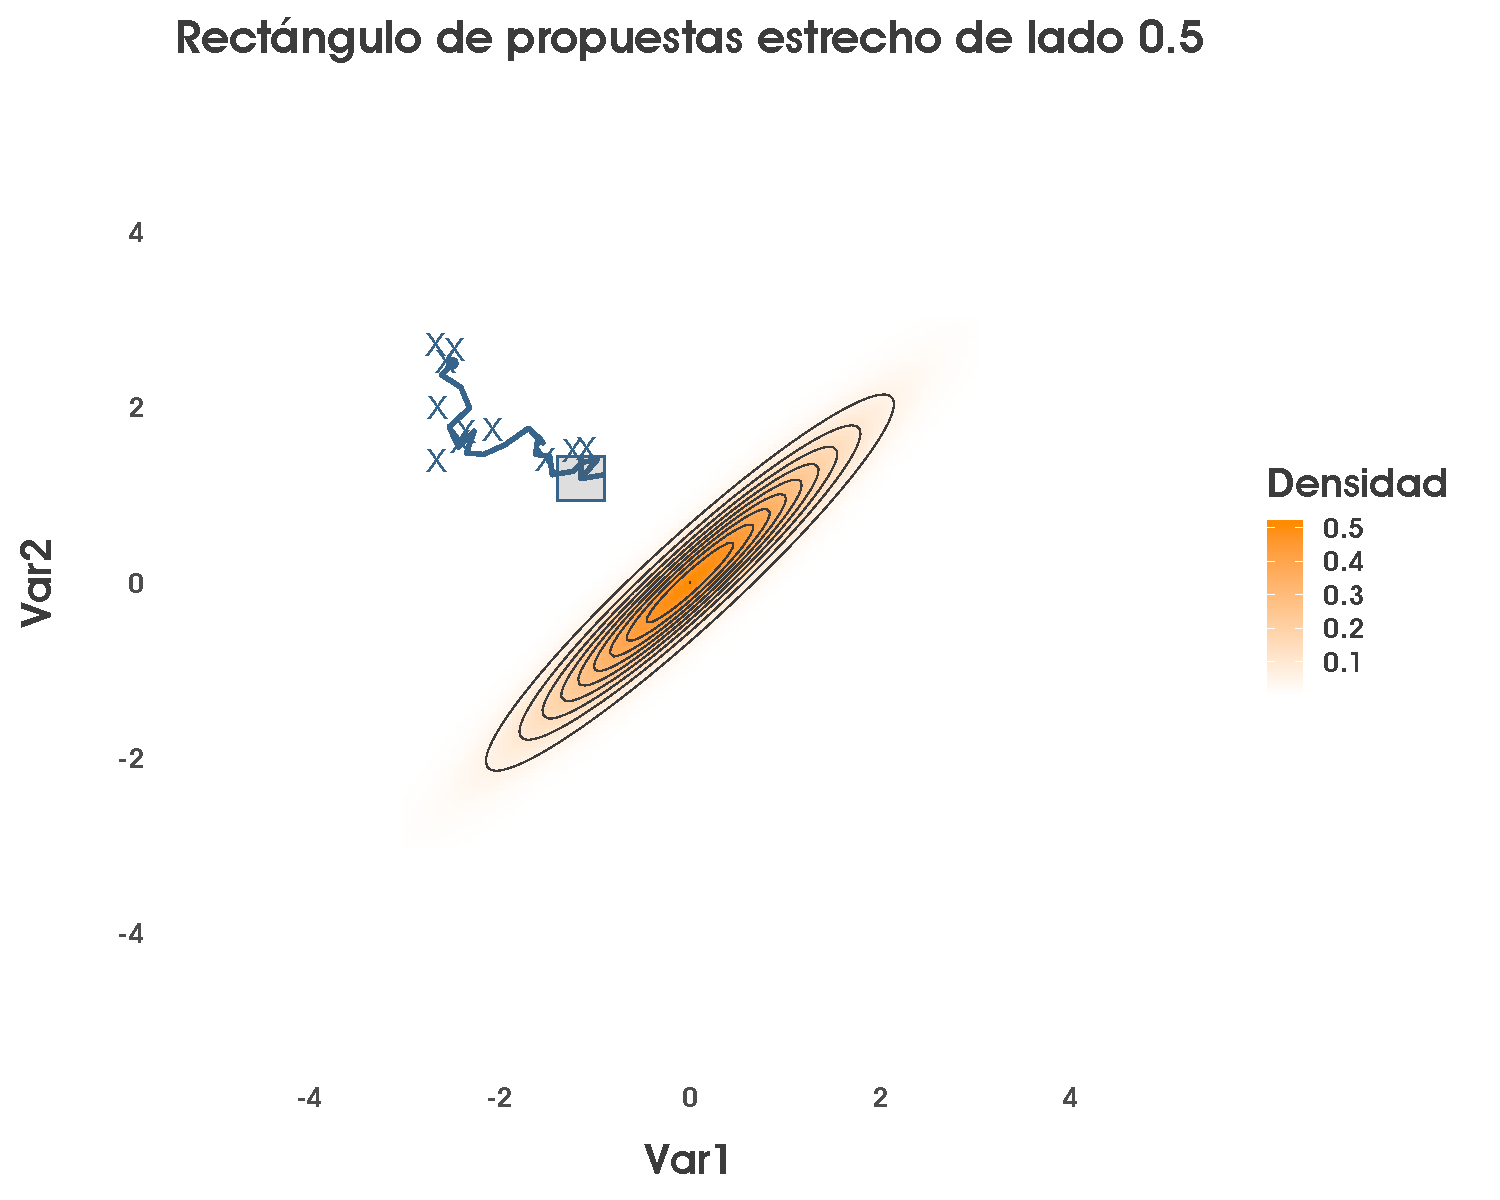
\includegraphics[width=\textwidth]{Figs/Bayes/Ejemplo_RWM_Compara1}
        \caption{El kernel de propuestas uniforme en un rectángulo de lado 3 centrado en el punto actual permite alcanzar puntos más distantes pero también propone valores frecuentemente rechazados al alejarse demasiado de la región crítica.}
    \end{subfigure}
    ~ 
    \begin{subfigure}{0.3\textwidth}
        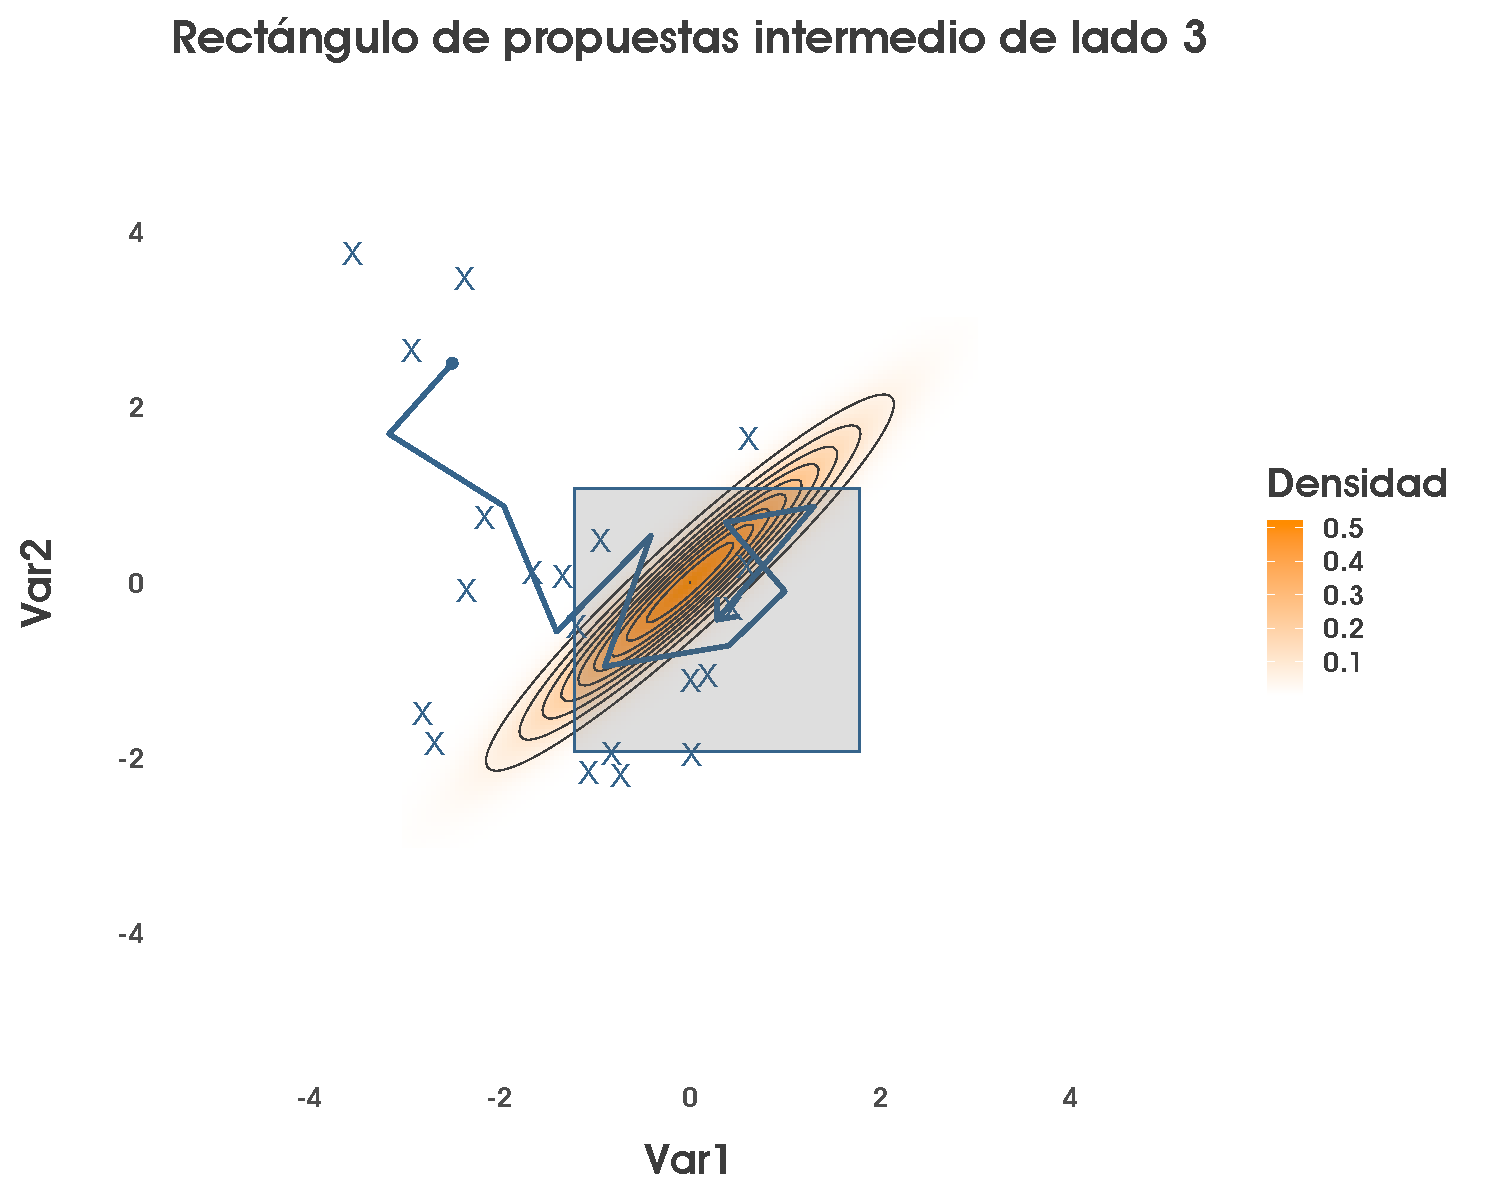
\includegraphics[width=\textwidth]{Figs/Bayes/Ejemplo_RWM_Compara2}
        \caption{El kernel de propuestas uniforme en un rectángulo de lado 0.5 centrado en el punto actual propone valores normalmente aceptados pero avanza lentamente.}
    \end{subfigure}
    ~
    \caption{Comparación de dos kerneles uniformes de propuestas para simular una normal bivariada correlación $0.95$ mediante RWM. Fuente: elaboración propia.}\label{fig:RWM_Corr}
\end{figure}

Ambas cadenas convergerán, pero este ejemplo ilustra uno de los principales problemas de los algoritmos de MH, en general. Elegir un kernel de propuestas eficiente no es sencillo. Ciertamente hay investigación enfocada a proponer ``reglas de dedo'' que funcionen \parencites{Geyer05,}, Más aún, la dimensionalidad de los problemas hace que muy rápidamente nos alejemos de los ejemplos triviales y seamos incapaces de proponer kérneles de transición que funcionen de manera adecuada. ¿Qué hacer? Por varios años se tuvieron que encontrar soluciones \textit{ad hoc}, hasta la década de los 90 cuando hubo una ``epifanía'' en el mundo de la estadística bayesiana \parencite{RobertCasella11}. 

\subsection{Gibbs Sampler}

\textcite{GelfandSmith90} presentaron en 1990. 

\section{Hamiltonian Monte Carlo}